\documentclass[twoside, a4paper]{article}
\usepackage[inner=2cm, outer=2cm, top=2cm, bottom=2cm, includeheadfoot]{geometry} 

\raggedbottom
% \raggedleft
% \raggedright
\usepackage[most]{tcolorbox}
% \usepackage{amsmath}
\usepackage{amssymb}
\usepackage{shortcut}
\usepackage{graphicx}
\usepackage{tabularx}
\usepackage{hyperref}

\renewcommand{\familydefault}{\sfdefault }

\title{ Njang/jàng Xayma}
\author{SARR Georges Mbissane}
\date{Ci wéeru ñaari junni ak ñaar fukk ak ñaar (2022)}


\begin{document}

\maketitle

Téeré ak video yi top la sukëndiku ngir bind téeré xayma bi:
\begin{itemize}
  \item \href{https://www.youtube.com/@ecolesausenegal/search?query=cours%20mathematiques%20wolof}{Youtube: Ecoles au Senegal, Cours - Mathématiques - Wolof *}
  \item \href{https://fr.glosbe.com/}{Baatukaay ci biir internet}
  \item \href{https://ia801303.us.archive.org/29/items/dictionnairesfra00holy/dictionnairesfra00holy.pdf}{Dictionnaire Wolof-Français, Français-Wolof} (baatukay bu magét la nak)
  \item Téeré xayma wu David Delaunay CPGE Dupuy Delome
\end{itemize}

% Ay baat you am solo:
% \begin{itemize}
%     \item jéemantu: exercice ?
%     \item njumté: erreur
%     \item lim: compter/nombre
%     \item mandargal: représenter ? -> royukaay ? (exemple) 30 moy mandargal fanweer
%     \item nguir leeraal: pour expliquer
%     \item saam: ensemble ?
%     \item këraleg: tableau ?
%     \item tontu: réponse
%     \item nafar: souvenir ? en lien avec nafa -> Bourse, Poche, Porte-feuille (objet qui permet de garder un autre objet)
%     \item tegtal ? : indication ?
%     \item nataal: image
%     \item njem: entreprise dans le sens d'entreprendre ?
%     \item jumtukaay: outil
%     \item xaymakaay/jumtukaay xayma: calculatrice
%     \item cax: devinette/problème ? exemple: (caxu Xayma) problème en mathématiques
%     \item ac/toxal: retenue (dans les opérations arithmétiques)
%     \item tomb: point
%     \item ëmbef: élément ?
%     \item mboolo: group
%     \item $a$ ñu toftal ci $b$: on met $b$ après $a$ ? 
% \end{itemize}

\section{Ëmb}
\begin{tcolorbox}[enhanced jigsaw,breakable,pad at break*=1mm,
    colback=red!5!white,colframe=white!75!black,title= Téeki,
    watermark color=white]
  Nañu wowee ëmb, beep saamu cër\footnote{élément} yu ñuy wowee ëmbeef. Amal been ëmb $E$, da ñuy né $x$ ëmbeefu $E$ la, ta ñu ko bindé $x\in E$\footnote{Mën na ñu ko liré "$x$ mu ngi ci biir $E$"}, bu féké ni $x$ ci biir $E$ la nek/la bok.
\end{tcolorbox}

\begin{itemize}
  \item $\N, \Z, \Q, \R$ ay ëmb la ñu.
  \item $\{a, b, c, d, ... z\}$ moy ëmb bu am ab ëmbeef $a$, $b$, $c$, ..., ba $z$
  \item $\emptyset$ moy mbindu ëmb bu amul tus, manam ëmb bu amul been ëmbeef.
  \item $\{a, b\} = \{b, a\}$
\end{itemize}
\begin{figure}[ht]
  \centering
  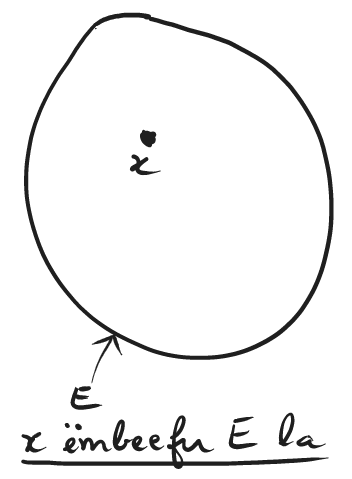
\includegraphics[scale = 0.5]{image/embeefu_emb.png}
  % \caption{}
  \label{fig:embeefu_emb}
\end{figure}



\subsection{Wàllu ëmb}
\begin{tcolorbox}[enhanced jigsaw,breakable,pad at break*=1mm,
    colback=red!5!white,colframe=white!75!black,title= Téeki,
    watermark color=white]
  Amal ëmb $E$ ak ëmb $F$, $E$ mu ngi ci biir $F$ bu féké ni rek\footnote{si et seulement si = bu féké ni rek ?} ëmbeef $x$ yëp yu nek ci $E$ ñu ngi ci biir $F$. Da ñuy wax itam $E$ wàllu $F$ la, di ko bindé $E \subset F$.
\end{tcolorbox}

Nañu mandargal wàllu ëmb:
\begin{itemize}
  \item Amal ëmb $E=\{1,2,3\}$, $F=\{1,2,3,4,5,6\}$ ak $G = \{1,2,4,5,6\}$, kon $E \subset F$, wayé $E$ nekkoul wàllu $G$, ñu koy bindé $E\not\subset G$, ndaxté $3$ mu ngi ci biir $E$, wanté $3$ nekkul ci biir $G$.
\end{itemize}
\begin{figure}[ht]
  \centering
  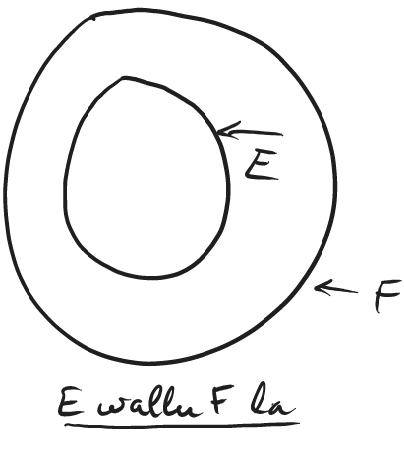
\includegraphics[scale = 0.5]{image/wallu_emb.png}
  % \caption{}
  \label{fig:wallu_emb}
\end{figure}


\subsection{Ëmbu ay wàllu been ëmb}
\begin{tcolorbox}[enhanced jigsaw,breakable,pad at break*=1mm,
    colback=red!5!white,colframe=white!75!black,title= Téeki,
    watermark color=white]
  Amal been ëmb $E$, ëmbu wàllu $E$ yi, mo di saamu wàllu $E$ yëp, ñu di ko bindé $\mathcal{W}(E)$.
\end{tcolorbox}

Nañu mandargal ëmbu ay wàllu been ëmb:
\begin{itemize}
  \item Amal ëmb $E=\{a,b,c\}$, $\mathcal{W}(E) = \big\{\emptyset, \{a\}, \{b\}, \{c\}, \{a,b\}, \{a,c\}, \{b,c\}, \{a,b,c\}\}\big\}$
\end{itemize}

\begin{tcolorbox}[enhanced jigsaw,breakable,pad at break*=1mm,
    colback=yellow!5!white,colframe=white!75!black,title= Seetlu,
    watermark color=white]
  \begin{itemize}
    \item Amal been ëmb $E$: $E\subset E$\footnote{ñu di ko bindé itam  $E \in\mathcal{W}(E)$}, manaam $E$ wàllu $E$ la
    \item Ëmbeefu $\mathcal{W}(E)$ ay ëmb la ñu.
  \end{itemize}
\end{tcolorbox}


\subsection{Sëfu Xayma ci ëmb yi}
\subsubsection{Selebe(yoon) ay ëmb (intersection d'ensembles)}

\begin{tcolorbox}[enhanced jigsaw,breakable,pad at break*=1mm,
    colback=red!5!white,colframe=white!75!black,title= Téeki,
    watermark color=white]
  Amal ëmb $E$ ak ëmb $F$, saamu ëmbeef $x$ yëp yu bok ci $E$ té bok itam ci $F$, ñu di ko bindé $E \cap F$  la ñuy wowee selebe wu $E$ ak $F$
\end{tcolorbox}

Nañu mandaargal\footnote{Exemple ?} selebe ay ëmb.
\begin{itemize}
  \item Amal  ñaari ëmb $E = \{1,2,3\}$ ak $F=\{4,5\}$, $E \cap F = \emptyset$ (manaam $E$ ak $F$ bokku ñu been ëmbeef.)
  \item Amal $E = \emptyset = F$, $E \cap F = \emptyset$
  \item Amal $E = \emptyset$, $F = \{0,1\}$, $E \cap F = \emptyset$
\end{itemize}

\subsubsection{Lëkkalé/Mboole ay ëmb (union d'ensembles)}

\begin{tcolorbox}[enhanced jigsaw,breakable,pad at break*=1mm,
    colback=red!5!white,colframe=white!75!black,title= Téeki,
    watermark color=white]
  Amal ëmb $E$ ak ëmb $F$, saamu ëmbeef $x$ yëp yu bok ci $E$ wala bok ci $F$, ñu di ko bindé $E \cup F$  la ñuy wowee mboolo $E$ ak $F$.
\end{tcolorbox}

Nañu mandaargal mbollo ëmb:
\begin{itemize}
  \item Amal  ñaari ëmb $E = \{1,2,3,4,5\}$ ak $F=\{4,5,6,7,8,9\}$, $E \cup F =\{1,2,3,4,5,6,7,8,9,10\}$
  \item Amal $E = \emptyset = F$, $E \cup F = \emptyset$
  \item Amal $E = \emptyset$, $F = \{0,1\}$, $E \cup F = \{0,1\}$
\end{itemize}

\begin{figure}[ht]
  \centering
  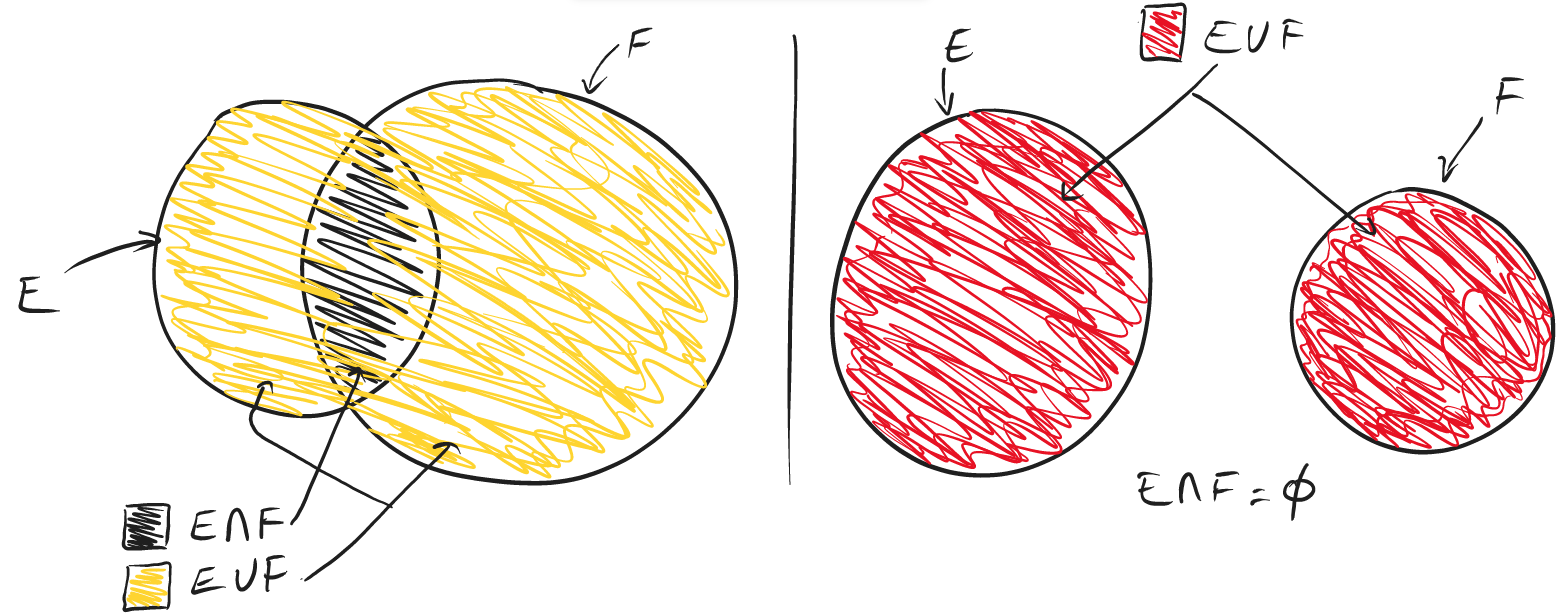
\includegraphics[scale = 0.5]{image/mbollo_selebe_emb.png}
  % \caption{}
  \label{fig:mbollo_selebe_emb}
\end{figure}


\subsubsection{Full carteseng ay ëmb}
\begin{tcolorbox}[enhanced jigsaw,breakable,pad at break*=1mm, colback=red!5!white,colframe=white!75!black,title= Téeki,
    watermark color=white]
  Amal ñaari ëmb $E$ ak $F$, fullu $E$ ak $F$, ñu koy bindé $E \times F$, mo di beep tank-tank\footnote{couple} $(x,y)$ bu deme ni\footnote{tel que} $x \in E$ ak $y\in F$
\end{tcolorbox}

\begin{itemize}
  \item Amal $E=\{1,2,3\}$ ak $F = \{4,5\}$, kon $E\times F =\big\{(1,4), (1,5), (2,4), (2,5), (3,4), (3,5)\big\}$
\end{itemize}


\begin{tcolorbox}[enhanced jigsaw,breakable,pad at break*=1mm, colback=red!5!white,colframe=white!75!black,title= Téeki,
    watermark color=white]
  Amal been limukaay $n \in \N$ bu eup $2$\footnote{$n\geq 2$}. Amal itam $n$ ëmb $E_1, E_2, ..., E_n$, fullu $E_1, E_2, ..., E_n$, ñu koy bindé $E_1 \times ... \times E_n$, mo di beep ëmbeef $x = (x_1,..,x_n)$ bu deme ni\footnote{tel que} $x_1 \in E_1$, $x_2 \in E_2$, ..., $x_n \in E_n$
\end{tcolorbox}


\begin{tcolorbox}[enhanced jigsaw,breakable,pad at break*=1mm,
    colback=yellow!5!white,colframe=white!75!black,title= Seetlu,
    watermark color=white]
  Amal ëmb $E$ ak ëmb $F$;
  \begin{itemize}
    \item Bu féké $E$ ak $F$ ay ëmb yu wuté la ñu, ñuy binde $E\neq F$, té itam $E\neq \emptyset$ ak $F\neq \emptyset$, kon fullu $E$ ak $F$ wuté na ak fullu $F$ ak $E$, ñuy bind $E\times F \neq F \times E$
    \item Bu féké $E = F$, manaam $E$ ak $F$ been la ñu, mën na ñu binde $E\times F = E \times E = E^2$
    \item Amal ñaari tank-tank $(u, v)$ ak $(x, y)$ ci biir $E\times F$, da ñuy né $(u, v) = (x, y)$ bu féké rek $u = x$ ak $v = y$. Ngir leeral, $(1,2) \in \N^2$ ak $(1,3)\in \N^2$ wuté na ñu, ndaxté $2$ wuté na ak $3$.
    \item Bu féké ni limu ëmbeefu $E$ ak limu ëmbeefu $F$ da ñuy jex\footnote{$E$ et $F$ sont des ensembles finis.}, kon ëmbeefu $E\times F$ maat nañu lu tolu ci limu ëmbeefu $E$ nga ful ko ak limu ëmbeefu $F$. Ngir leeral wax ji, amal $E=\{1,2,3\}$ ak $F = \{4,5\}$, kon $E$ amna ñaat ëmbeef (kon limu ëmbeefu $E$, manam ñaat, day jex), $F$ amna ñaari ëmbeef (kon limu ëmbeefu $F$, manam ñaar, day jex), limu ëmbeefu $E\times F$ mo di ñaat nga full ko ak ñaar, manaan $3\times 2=6$. Leneen lu koy woné mo di: $E\times F =\big\{(1,4), (1,5), (2,4), (2,5), (3,4), (3,5)\big\}$ amna bu bax juròom-been (6) ëmbeef.
  \end{itemize}
  \begin{itemize}
    \item Amal $n$ ëmb $E_1, E_2, ..., E_n$, bu féké ni $E=E_1=E_2=...=E_n$, mên na ñu binde,  $E_1 \times ... \times E_n = E^n$
  \end{itemize}
\end{tcolorbox}


\begin{figure}[ht]
  \centering
  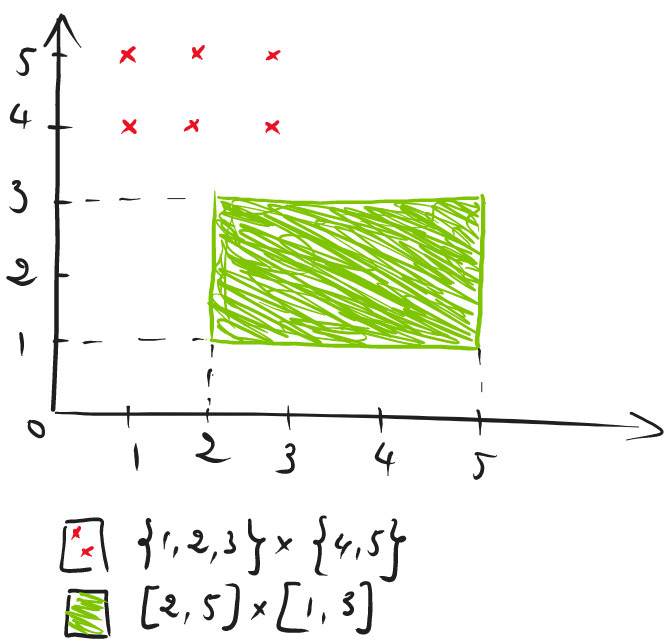
\includegraphics[scale = 0.5]{image/full_carteseng.png}
  % \caption{}
  \label{fig:full_carteseng}
\end{figure}


\section{Doxalin}
\begin{tcolorbox}[enhanced jigsaw,breakable,pad at break*=1mm, colback=red!5!white,colframe=white!75!black,title= Téeki,
    watermark color=white]
  Been \footnote{Fonction ou application}doxalin $f$ mo di beep ñaati ëmb $E$, $F$ ak $\mathcal{G}$. $E$ moy ëmbef bu doxalin $f$ di tambali, $F$ moy ëmbef bu muy agsi.
  Da ñuy bindë $\mathcal{G} = \big\{ (x,y) \in E\times F, y = f(x)\big\}$.
  Ëmb $\mathcal{G}$, ñu di ko wowé graaf, moy lëkkalé beep ëmbeef $x\in E$ ak been ëmbeef $y\in F$ rek. Doxalin $f$ ñio ngi koy bindé: $$f: \left\{
    \begin{array}{ll}
      E \rightarrow{} F \\
      x \mapsto f(x)
    \end{array}
    \right.$$
  wala ñuy binde $$f: E \rightarrow F, \hspace{0.2cm}\text{ak } f(x) = ...$$

  wala itam $$f: x\mapsto ... \hspace{0.2cm} \hspace{0.2cm} \text{ak } f: E \rightarrow F$$\\
  Beep ëmbeef $x\in E$ warna am been natal\footnote{Image par une fonction} rek ci $f$, nataal gogu  ñu di ko bindé $f(x)$
\end{tcolorbox}

Nañu binde $\R_{+} = \{x \in \R, x \geq 0 \}$ manaam ëmbeefu limu $\R$ yu "positif" yi walla tolo ak tus, ak $\R_{+}^{*} = \{x \in \R, x > 0 \}$, manaam ëmbeefu limu $\R$ yu "positif" yi té weesu/ëp tus.

\begin{itemize}
  \item Doxalin $f: \left\{
          \begin{array}{ll}
            \R \rightarrow{} \R \\
            x \mapsto x^2+1
          \end{array}
          \right.$ ak doxalin $g: \left\{
          \begin{array}{ll}
            \R \rightarrow{} \R_{+} \\
            x \mapsto x^2+1
          \end{array}
          \right.$ wuté nañu, ndaxté ëmbeef yu ñuy agsi wuté nañu: $\R \neq \R_{+}$

  \item $f: \left\{
          \begin{array}{ll}
            \R \rightarrow{} \R_{+}^{*} \\
            x \mapsto x^2
          \end{array}
          \right.$ nekkul doxalin, ndaxté $0^2=0\not\in \R_{+}^{*}$
\end{itemize}


\section{Xalaat ci Xayma}

\subsection{Baat}
\begin{tcolorbox}[enhanced jigsaw,breakable,pad at break*=1mm, colback=red!5!white,colframe=white!75!black,title= Téeki,
    watermark color=white]
  Been \textbf{baat}\footnote{assertion, prédicat} ci Xayma mo di beep kaadu gi mëna nekka dëgg\footnote{vrai}, walla nekka lu dul dëgg\footnote{faux}.\\
  Dëgg (D), ak lu dëggul (L) la ñuy wowee xayma dëgg\footnote{valeur de vérité}. Bu féké ñaari baat $\mathcal{B}$ ak $\mathcal{C}$ ño bok xayma dëgg, kon da ñuy né ño niro, di ko bindé: $\mathcal{B}\sim \mathcal{C}$, seeni xayma dëg bu ñu wuté wé, da ñuy bindë $\mathcal{B}\not\sim \mathcal{C}$
\end{tcolorbox}
Amal  $(0,1,2)\in \N^3$, kon baat $\mathcal{B} = "1 \geq 0"$ dëgg la, wanté, baat $\mathcal{C} = "2 + 1 \leq 2"$ du dëgg, kon bok $\mathcal{B}\not\sim \mathcal{C}$.\\
Baat $\mathcal{B}="2=0"$ ak baat $\mathcal{C}="1>2"$ dëgguñu, kon $\mathcal{B}\sim \mathcal{C}$.


\subsection{Muk/Deet}
\begin{tcolorbox}[enhanced jigsaw,breakable,pad at break*=1mm, colback=red!5!white,colframe=white!75!black,title= Téeki,
    watermark color=white]
  \textbf{Muk been baat}\footnote{La négation d'une assertion}$\mathcal{B}$, ñu di ko bindé $\textit{muk } \mathcal{B}$ (wala $\neg  \mathcal{B}$) baatu dëgg la, bu féké ni $\mathcal{B}$ du dëgg. Té itam, baat bu dëggul la, bu féké ni $\mathcal{B}$ dëgg la.
\end{tcolorbox}
Amal $x \in \R$, $\mathcal{B}(x) = " x \leq 0"$, kon $\neg \mathcal{B}(x) \sim "x > 0"$.

\begin{tcolorbox}[enhanced jigsaw,breakable,pad at break*=1mm, colback=blue!5!white,colframe=white!75!black,title= Tèg\footnote{Proposition},
    watermark color=white]
  Amal been baat $\mathcal{B}$, boba/kon $\neg (\neg \mathcal{B}) \sim \mathcal{B}$, manaam muk (muk $\mathcal{B}$) ak $\mathcal{B}$ ño book xayma dëgg.
\end{tcolorbox}

\textbf{Woné:}
\vspace{0.3cm}
Amal been baat $\mathcal{B}$ \newline
\vspace{0.3cm}
\begin{tabularx}{0.8\textwidth} {
    | >{\centering\arraybackslash}X
    | >{\centering\arraybackslash}X
    | >{\centering\arraybackslash}X |}
  \hline
  $\mathcal{B}$ & $\neg\mathcal{B}$ & $\neg(\neg\mathcal{B})$ \\
  \hline
  D             & L                 & D                       \\
  L             & D                 & L                       \\
  \hline
\end{tabularx}

\subsection{Takhalé ak tékhalé ay baat}
\begin{tcolorbox}[enhanced jigsaw,breakable,pad at break*=1mm, colback=red!5!white,colframe=white!75!black,title= Téeki\footnote{Définition},
    watermark color=white]
  Takhalo\footnote{Conjonction} ñaari baat $\mathcal{B}$ ak $\mathcal{C}$, ñu di ko bindé $\mathcal{B}\hspace{0.1cm}\land\hspace{0.1cm}\mathcal{C}$, wala $\mathcal{B} \textit{ ak } \mathcal{C}$, baatu dëgg la bu féké ni rek $\mathcal{B}$ dëgg la, té $\mathcal{C}$ dëgg la itam.\\

  Tékhalo\footnote{Disjonction} ñaari baat $\mathcal{B}$ ak $\mathcal{C}$, ñu di ko bindé $\mathcal{B}\hspace{0.1cm}\lor\hspace{0.1cm}\mathcal{C}$, wala $\mathcal{B} \textit{ wala } \mathcal{C}$, dëgg la bu féké ni rek $\mathcal{B}$ dëgg la, wala $\mathcal{C}$ dëgg la.\\

  \begin{tabularx}{0.8\textwidth} {
      | >{\centering\arraybackslash}X
      | >{\centering\arraybackslash}X
      | >{\centering\arraybackslash}X
      | >{\centering\arraybackslash}X |}
    \hline
    $\mathcal{B}$ & $\mathcal{C}$ & $\mathcal{B}\hspace{0.1cm}\land\hspace{0.1cm}\mathcal{C}$ & $\mathcal{B}\hspace{0.1cm}\lor\hspace{0.1cm}\mathcal{C}$ \\
    \hline
    D             & D             & D                                                         & D                                                        \\
    D             & L             & L                                                         & D                                                        \\
    L             & D             & L                                                         & D                                                        \\
    L             & L             & L                                                         & L                                                        \\
    \hline
  \end{tabularx}
\end{tcolorbox}


\begin{tcolorbox}[enhanced jigsaw,breakable,pad at break*=1mm, colback=blue!5!white,colframe=white!75!black,title= Tèg\footnote{Proposition},
    watermark color=white]
  Amal baat $\mathcal{B}$ ak baat $\mathcal{C}$, boba/kon:
  $$\neg(\mathcal{B} \land \mathcal{C}) \sim (\neg\mathcal{B}) \lor (\neg \mathcal{C})$$
  $$\neg(\mathcal{B} \lor \mathcal{C})\sim (\neg\mathcal{B}) \land (\neg \mathcal{C})$$
\end{tcolorbox}

\textbf{Woné:}

Amal baat $\mathcal{B}$ ak baat $\mathcal{C}$, nañu bindë këralegu/natalu\footnote{tableau ?} xayma dëgg baat yi.\\

\begin{tabularx}{0.8\textwidth} {
    | >{\centering\arraybackslash}X
    | >{\centering\arraybackslash}X
    | >{\centering\arraybackslash}X
    | >{\centering\arraybackslash}X
    | >{\centering\arraybackslash}X
    | >{\centering\arraybackslash}X |}
  \hline
  $\mathcal{B}$ & $\mathcal{C}$ & $\neg\mathcal{B}\hspace{0.1cm}\lor\hspace{0.1cm}\neg\mathcal{C}$ & $\neg(\mathcal{B}\hspace{0.1cm}\land\hspace{0.1cm}\mathcal{C})$ & $\neg(\mathcal{B}\hspace{0.1cm}\lor\hspace{0.1cm}\mathcal{C})$ & $(\neg\mathcal{B})\hspace{0.05cm}\land\hspace{0.05cm}(\neg\mathcal{C})$ \\
  \hline
  D             & D             & L                                                                & L                                                               & L                                                              & L                                                                       \\
  D             & L             & D                                                                & D                                                               & L                                                              & L                                                                       \\
  L             & D             & D                                                                & D                                                               & L                                                              & L                                                                       \\
  L             & L             & D                                                                & D                                                               & D                                                              & D                                                                       \\
  \hline
\end{tabularx}

Mën nañu gis ci ñaatel jeñ\footnote{Colonne = jiñ = jeñ ?} gi ak ñeentel gi, né $\neg(\mathcal{B} \land \mathcal{C}) \sim (\neg\mathcal{B}) \lor (\neg \mathcal{C})$. Juròomeel jeñ gi ak juròomeel-beeneel gi, woné nañu né $\neg(\mathcal{B} \lor \mathcal{C})\sim (\neg\mathcal{B}) \land (\neg \mathcal{C})$.


\begin{tcolorbox}[enhanced jigsaw,breakable,pad at break*=1mm, colback=green!5!white,colframe=white!75!black,title= Tègtal\footnote{Indication ?},
    watermark color=white]
  Ngir woné né ñaari baat ño bok xayma dëgg, mën naño jëfandikoo këralegu xayma dëgg yi.
\end{tcolorbox}

\textbf{Jéemantu}\\
Amal ñaat baat $\mathcal{A}, \mathcal{B}, \mathcal{C}$, wonéel ni:
\begin{align*}
  \mathcal{B} \land \mathcal{B}                     & \sim \mathcal{B}                                                          \\
  \mathcal{B} \lor \mathcal{B}                      & \sim \mathcal{B}                                                          \\
  (\mathcal{B} \land \mathcal{C}) \land \mathcal{A} & \sim \mathcal{B} \land (\mathcal{C} \land \mathcal{A})                    \\
  (\mathcal{B} \lor \mathcal{C}) \lor \mathcal{A}   & \sim \mathcal{B} \lor (\mathcal{C} \lor \mathcal{A})                      \\
  (\mathcal{B} \land \mathcal{C}) \lor \mathcal{A}  & \sim (\mathcal{B} \lor \mathcal{A}) \land (\mathcal{C} \lor \mathcal{A})  \\
  (\mathcal{B} \lor \mathcal{C}) \land \mathcal{A}  & \sim (\mathcal{B} \land \mathcal{A}) \lor (\mathcal{C} \land \mathcal{A})
\end{align*}

\subsection{Baat bi yobualé/andi been baat}
\begin{tcolorbox}[enhanced jigsaw,breakable,pad at break*=1mm, colback=red!5!white,colframe=white!75!black,title= Téeki,
    watermark color=white]
  Amal baat $\mathcal{B}$ ak baat $\mathcal{C}$. Da ñuy né $\mathcal{B}$ \textit{da yobualé  }$\mathcal{C}$\footnote{$\mathcal{B}$ implique $\mathcal{C}$} dëgg la, bu féké ni rek $\mathcal{C}$ mënul bagna nek dëgg bu $\mathcal{B}$ néké dëgg.\\
  $\mathcal{B}$ \textit{da yobualé  }$\mathcal{C}$  ñu di ko bindé $\mathcal{B} \implies \mathcal{C}$.\\

  Xayma dëgg $\mathcal{B} \implies \mathcal{C}$ mu ngi ni:\\

  \begin{tabularx}{0.8\textwidth} {
      | >{\centering\arraybackslash}X
      | >{\centering\arraybackslash}X
      | >{\centering\arraybackslash}X |}
    \hline
    $\mathcal{B}$ & $\mathcal{C}$ & $\mathcal{B}\implies\mathcal{C}$ \\
    \hline
    D             & D             & D                                \\
    D             & L             & L                                \\
    L             & D             & D                                \\
    L             & L             & D                                \\
    \hline
  \end{tabularx}
\end{tcolorbox}

Ak beep $x\in\R$, bo bindé $\mathcal{B}(x) = "x >= 2"$, $\mathcal{C}(x) = "x^2 >= 4"$, kon $\mathcal{B}(x) \implies \mathcal{C}(x)$ dëgg la.


\begin{tcolorbox}[enhanced jigsaw,breakable,pad at break*=1mm, colback=red!5!white,colframe=white!75!black,title= Téeki,
    watermark color=white]
  Bu $\mathcal{B} \implies \mathcal{C}$ néké dëgg, kon da ñuy né
  \begin{itemize}
    \item $\mathcal{B}$ \textit{baat bu doy} $\mathcal{C}$ la, wala $\mathcal{B}$ \textit{doy na} $\mathcal{C}$.\footnote{$\mathcal{B}$ est une condition suffisante pour $\mathcal{C}$}
    \item $\mathcal{B}$ \textit{da soxla} $\mathcal{C}$.\footnote{$\mathcal{C}$ est une condition nécessaire pour $\mathcal{B}$}
  \end{itemize}

  $\mathcal{C} \implies \mathcal{B}$ mo di \textit{wëlbati wu} \footnote{implication réciproque} baat $\mathcal{B} \implies \mathcal{C}$.
\end{tcolorbox}



\begin{tcolorbox}[enhanced jigsaw,breakable,pad at break*=1mm, colback=blue!5!white,colframe=white!75!black,title= Tèg\footnote{Proposition},
    watermark color=white]
  Amal baat $\mathcal{B}$ ak baat $\mathcal{C}$, boba:
  \begin{align*}
    (\mathcal{B} \implies \mathcal{C}) & \sim (\neg\mathcal{B}) \lor \mathcal{C}                        \\
    (\mathcal{B} \implies \mathcal{C}) & \sim \big( (\neg\mathcal{C}) \implies (\neg \mathcal{B}) \big)
  \end{align*}

  $(\neg\mathcal{C}) \implies (\neg \mathcal{B})$ la ñuy wowee \textit{contaraposee}\footnote{Contraposée} wu $\mathcal{B} \implies \mathcal{C}$
\end{tcolorbox}

\textbf{Woné:}

\begin{tabularx}{0.8\textwidth} {
    | >{\centering\arraybackslash}X
    | >{\centering\arraybackslash}X
    | >{\centering\arraybackslash}X
    | >{\centering\arraybackslash}X |}
  \hline
  $\mathcal{B}$ & $\mathcal{C}$ & $\mathcal{B}\implies\mathcal{C}$ & $(\neg\mathcal{B}) \lor \mathcal{C}$ \\
  \hline
  D             & D             & D                                & D                                    \\
  D             & L             & L                                & L                                    \\
  L             & D             & D                                & D                                    \\
  L             & L             & D                                & D                                    \\
  \hline
\end{tabularx}
\vskip 0.5cm
Mën na ñu gis né $(\mathcal{B} \implies \mathcal{C}) \sim (\neg\mathcal{B}) \lor \mathcal{C}$ ci ñaateel jeñ ak ñeenteel gi, kon bok bu ñu wécanté $\mathcal{B}$ ak $\neg \mathcal{C}$, té wécanté itam $\mathcal{C}$ ak $\neg\mathcal{B}$, ñu am $\big( (\neg\mathcal{C}) \implies (\neg \mathcal{B}) \big) \sim \big( (\neg(\neg\mathcal{C})) \lor (\neg\mathcal{B})\big) \sim \big(\mathcal{C} \lor (\neg\mathcal{B}) \big)\sim (\neg\mathcal{B}) \lor \mathcal{C} \sim (\mathcal{B} \implies \mathcal{C})$, fi la ñuy jexalé woné gi.\\

Mënon nañu woné itam
$(\mathcal{B} \implies \mathcal{C}) \sim \big( (\neg\mathcal{C}) \implies (\neg \mathcal{B}) \big)$ ak natal xayma dëgg yi.

\subsection{Baat yu yèm}
\begin{tcolorbox}[enhanced jigsaw,breakable,pad at break*=1mm, colback=red!5!white,colframe=white!75!black,title= Téeki,
    watermark color=white]
  Amal ñaari baat $\mathcal{B}$, $\mathcal{C}$.

  $\mathcal{B}$ \textit{mo yèm ak} $\mathcal{C}$\footnote{L'équivalence de deux assertions}, ñuy bindë $\mathcal{B}\iff \mathcal{C} $, mo di baat $(\mathcal{B}\implies \mathcal{C}) \land (\mathcal{C}\implies \mathcal{B})$, manaam $$\mathcal{B}\iff \mathcal{C} \sim \big( (\mathcal{B}\implies \mathcal{C}) \land (\mathcal{C}\implies \mathcal{B})\big) $$

  Natal xayma dëgg bu yèmalé ñaari baat mo ngi ni:\\\\

  \begin{tabularx}{0.8\textwidth} {
      | >{\centering\arraybackslash}X
      | >{\centering\arraybackslash}X
      | >{\centering\arraybackslash}X
      | >{\centering\arraybackslash}X
      | >{\centering\arraybackslash}X |}
    \hline
    $\mathcal{B}$ & $\mathcal{C}$ & $\mathcal{B}\implies\mathcal{C}$ & $\mathcal{C}\implies\mathcal{B}$ & $\mathcal{B}\iff\mathcal{C}$ \\
    \hline
    D             & D             & D                                & D                                & D                            \\
    D             & L             & L                                & D                                & L                            \\
    L             & D             & D                                & L                                & L                            \\
    L             & L             & D                                & D                                & D                            \\
    \hline
  \end{tabularx}\\\\
\end{tcolorbox}

\begin{tcolorbox}[enhanced jigsaw,breakable,pad at break*=1mm,
    colback=yellow!5!white,colframe=white!75!black,title= Seetlu,
    watermark color=white]
  Amal ñaari baat $\mathcal{B}$, $\mathcal{C}$.
  \begin{itemize}
    \item Bu $\mathcal{B}\iff\mathcal{C}$ néké dëgg, kon $\mathcal{B}\sim \mathcal{C}$.
    \item Bu féké $\mathcal{B}\iff\mathcal{C}$ dëggul, kon $\mathcal{B}\not\sim\mathcal{C}$
  \end{itemize}

  Seetlu yi muj, woné nañu né \textbf{yémalé ay baat ak nirolé lèn been lañu}. Manam wax $\mathcal{B}\iff\mathcal{C}$ been la ak wax $\mathcal{B}\sim \mathcal{C}$, manaam:
  \begin{align*}
    (\mathcal{B} \iff \mathcal{C}) & \sim \big( \mathcal{B} \sim \mathcal{C}\big) \\
    (\mathcal{B} \iff \mathcal{C}) & \iff \big( \mathcal{B} \sim \mathcal{C}\big)
  \end{align*}
\end{tcolorbox}
\begin{tcolorbox}[enhanced jigsaw,breakable,pad at break*=1mm, colback=blue!5!white,colframe=white!75!black,title= Tèg\footnote{Proposition},
    watermark color=white]
  Amal baat $\mathcal{B}$ ak baat $\mathcal{C}$, boba:
  \begin{align*}
    (\mathcal{B} \iff \mathcal{C}) & \sim \big( (\neg\mathcal{C}) \iff (\neg \mathcal{B}) \big)
  \end{align*}
\end{tcolorbox}

\textbf{Jéemantu:} Woneel tèg bi muj

\begin{tcolorbox}[enhanced jigsaw,breakable,pad at break*=1mm, colback=red!5!white,colframe=white!75!black,title= Téeki,
    watermark color=white]
  Bu $\mathcal{B} \iff \mathcal{C}$ néké dëgg, kon da ñuy né\\
  \begin{itemize}
    \item $\mathcal{B}$ \textit{baat bu soxla té doy} $\mathcal{C}$ la, \footnote{$\mathcal{B}$ est une condition nécessaire et suffisante pour $\mathcal{C}$}
  \end{itemize}
\end{tcolorbox}

\subsection{Natakat baat}

\begin{tcolorbox}[enhanced jigsaw,breakable,pad at break*=1mm, colback=red!5!white,colframe=white!75!black,title= Téeki,
    watermark color=white]
  Amal been ëmb $E$. Ak beep $x\in E$, amal been baat $\mathcal{B}(x)$ bu nék surgau $x$\footnote{Une assertion qui dépend de $x$}.

  Da ñuy wax \textit{ak beep $x\in E$, $\mathcal{B}(x)$ dëgg la}, té di bindë $$\forall x\in E, \mathcal{B}(x)$$ bu féké ni rek $\mathcal{B}(x)$ dëgg la ak beep ëmbeef $x$ bu nék ci biir $E$.\\

  Da ñuy wax \textit{ak been $x\in E$, $\mathcal{B}(x)$ dëgg la}, té di bindë $$\exists x\in E, \mathcal{B}(x)$$ bu féké ni rek $\mathcal{B}(x)$ dëgg la ak lu mu tuti tuti been ëmbeef $x$ bu nék ci biir $E$.\\

  Da ñuy wax \textit{ak been $x\in E$ rek, $\mathcal{B}(x)$ dëgg la}, té di bindë $$\exists! x\in E, \mathcal{B}(x)$$ bu féké ni rek $\mathcal{B}(x)$ dëgg la ak been ëmbeef $x$ dong bu nék ci biir $E$.
\end{tcolorbox}

Mën nañu né $\forall x \in \R, \exp(x) > 0$, ak $\forall x \in \R, \exists ! n \in \Z, n\leq x < n+1$\\

Amal been doxalin $f$ bi jogé ci $\R$ té agsi ci $\R$, kon bok:

Da ñuy wax $f$ moy doxalinu dara/tus \footnote{La fonction $f$ est la fonction nulle.} bu féké ni rek  $$\forall x \in \R, f(x) = 0$$
Da ñuy wax $f$ di na agsi ci tus\footnote{La fonction $f$ s'annule} bu féké ni rek $$\exists x \in \R, f(x) = 0$$
Da ñuy wax $f$ di na agsi been yoon ci tus bu féké ni rek \footnote{La fonction $f$ s'annule une seule fois} $$\exists! x \in \R, f(x) = 0$$
Da ñuy wax $f$ ci $\R_{+}$ rek la mëna tolo ak tus\footnote{La fonction $f$ ne s'annule que sur $\R_{+}$} bu féké ni rek $$\forall x \in \R, f(x) = 0 \implies x \in \R_{+}$$
wala itam $$\forall x \in \R, x \not\in \R_{+} \implies f(x) \neq 0$$


\begin{tcolorbox}[enhanced jigsaw,breakable,pad at break*=1mm, colback=blue!5!white,colframe=white!75!black,title= Tèg\footnote{Proposition},
    watermark color=white]
  \begin{align*}
    \neg(\forall x\in E, \mathcal{B}(x)) & \sim \exists x\in E, \neg \big(\mathcal{B}(x)\big) \\
    \neg(\exists x\in E, \mathcal{B}(x)) & \sim \forall x\in E, \neg \big(\mathcal{B}(x)\big)
  \end{align*}
\end{tcolorbox}
\textbf{Jéemantu:} Woneel tèg yi muj

\begin{tcolorbox}[enhanced jigsaw,breakable,pad at break*=1mm, colback=orange!5!white,colframe=white!75!black,title= Waxanté\footnote{Convention},
    watermark color=white]
  Beep baat buy tambalé ak $\exists x \in \emptyset$ dëggul, kon beep baat buy tambalé ak $\forall x \in \emptyset$ dëgg la.
\end{tcolorbox}

\textbf{Jéemantu bu am solo ci xam-xam ci koompuutar}\footnote{Exercice important en informatique}
Amal been doxalin $f$ bi jogé ci been full carteseng ëmb xayma dëgg yi $\{0,1\}^n$, té di agsi ci ëmbu xayma dëgg yi, $0$ di téeki lu dëggul $(L)$,  $1$ di téeki dëgg $(D)$, ñuy bindë
$$f: \{0,1\}^n \rightarrow \{0,1\}$$
mën nañu woné né $f$ mën nañu ko bindé ak sëfu xayma dëgg \textit{takhalo} (manaam $\land$) ak sëfu xayma dëgg \textit{deet} (manaam $\neg$). Manam bo jëlé $b = (b_1,b_2,...b_n) \in \{0,1\}^n$, kon $f(b)$ mën nañu kon bindé ak $b_1,b_2,...b_n$ ak $\land$ ak $\neg$ dong.\\
\textit{Tégtal: ngir woné tèg bi muj}
\begin{itemize}
  \item[$\bullet$] Mën nañ woné ni amna been $0\leq k \leq 2^n$ ak $f_1$, ..., $f_k$ ay doxalin yuy jogé ci $\{0,1\}^n$ té agsi ci $\{0,1\}$, yu mel ni $$f(b) = f^{(1)}(b) \lor f^{(2)}(b) \lor ... \lor f^{(k)}(b)$$ té $f^{(l)}(b) = \left\{\begin{array}{ll}
            1 \text{ bu féké ni $b=b^{(l)}$} \\
            0 \text{ bu féké ni $b\neq b^{(l)}$}
          \end{array}\right.$, ak $b^{(l)}$ been néekin $b$ ci këralegu xayma dëggu $f$, té $f(b^{(l)}) = 1$. Ngir léeral, bu féké $b=(1,0,1,0,0,0,1)$ ci liñ $l$ këralegu xayma dëgg doxalin $f$, té $f(b^{(l)}) = 1$, mën nañu bindë $b^{(l)} = (1,0,1,0,0,0,1)$ té bindë $f_l(b) = b_1 \land (\neg b_2) \land b_3 \land (\neg b_4) \land (\neg b_5) \land (\neg b_6) \land  b_7 $. Bu féké $f = 0$ (manaam $k=0$), kon mën nañu bindë $f(b)=b_1 \land (\neg b_1)$
  \item[$\bullet$] Fatéliku itam né $\lor$ mën nañu ko bindë ak $\land$ ak $\neg$
\end{itemize}
\begin{figure}[ht]
  \centering
  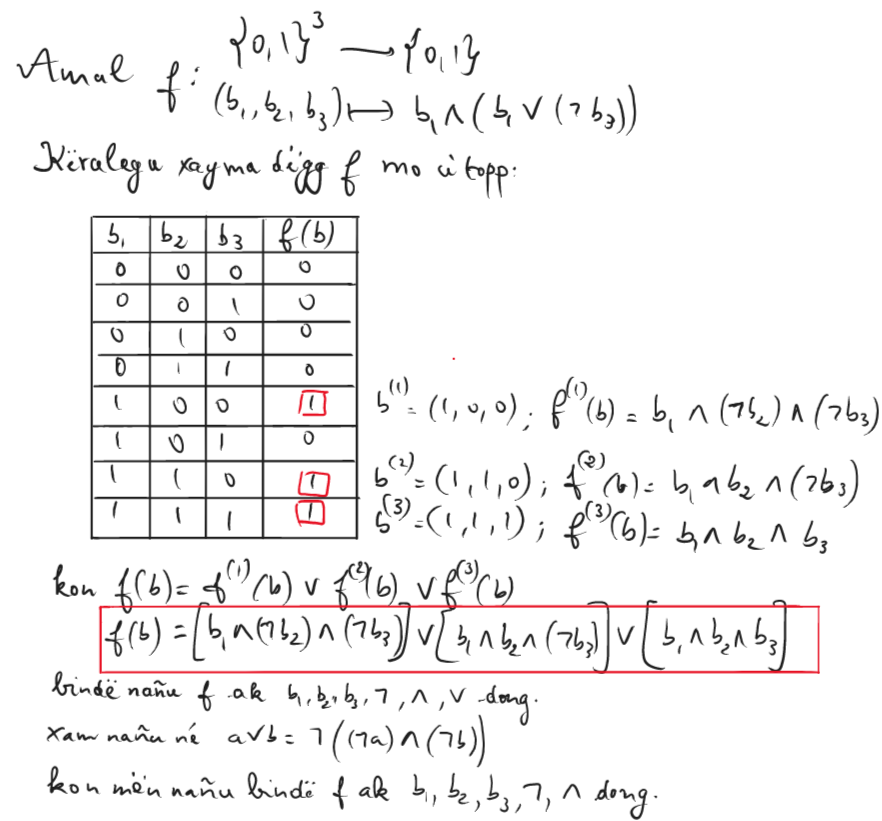
\includegraphics[scale = 0.5]{image/informatik0.png}
  % \caption{}
  \label{fig:informatik0}
\end{figure}


\subsection{Kadum sago}
Ngir wax né been baat, baatu dëgg la ci Xayma, war na ñu ko firndeel/woral ak been woné, manaam ci Xayma, woné rek moy dëggal been baat. Baatu dëgg bu nék, \textbf{tèg}\footnote{Proposition} la tud. Ci tèg yi, amna yu ci gëna am solo, ñu len di wowée \textbf{téorèm}\footnote{Théorème}. Wanté amna ay baat yu ñu dul woné té nangu né ay baati dëgg la ñu, ñu léen di wowée \textbf{ñalém}, wala \textbf{baatu dëga yu wor}\footnote{Axiomes}. Baat yoyu lé, mën na ñu lèna jappé ay sart\footnote{Règles} yuy lal xalaat ci Xayma.\\


Nañu lim woné yu ñuy tama jëfandiko ngir woral ay baat.

\subsubsection{Woné ab contaraposee}
\begin{tcolorbox}[enhanced jigsaw,breakable,pad at break*=1mm, colback=red!5!white,colframe=white!75!black,title= Téeki,
    watermark color=white]
  Mën na ñu woné been baat $\mathcal{B} \implies \mathcal{C}$ dëgg la, bu ñu woné  $(\neg\mathcal{C}) \implies (\neg \mathcal{B})$ dëgg la. Woné gi la ñuy wowée \textbf{woné contaraposee}\footnote{Démonstration par contraposition}


\end{tcolorbox}

\subsubsection{Tofal}

\begin{tcolorbox}[enhanced jigsaw,breakable,pad at break*=1mm, colback=red!5!white,colframe=white!75!black,title= Téeki,
    watermark color=white]
  Mën na ñu woné been baat $\mathcal{C}$ dëgg la, bu ñu tambali wé ci béneen baat $\mathcal{B}$ bu nek dëgg té woné ni $\mathcal{B} \implies \mathcal{C}$ dëgg la. Woné gi la ñuy wowée \textbf{tofal}\footnote{Tirer une conséquence.}.


\end{tcolorbox}




Nañu woné $$ \forall x \in \R, x^2 + 1 > 0$$ ak tofal.

Amal $x\in \R$. Xam na ñu $x^2 \geq 0$ ak $1 > 0$ wanté xamna ñu itam sa su jëlé $a$ ak $b$ ay ëmbeefu $\R$, $$(a \geq 0)\text{ ak }b > 0 \implies a+b >0$$ kon itam $x^2+1>0$ (bu ñu jëlé $a=x^2$ ak $b=1$).


\subsubsection{Tofal ak tékhalé ay baat / ak nékin yëp yu wuté}
\begin{tcolorbox}[enhanced jigsaw,breakable,pad at break*=1mm, colback=red!5!white,colframe=white!75!black,title= Téeki,watermark color=white]
  Mën nañu woné $\mathcal{C}$ dëgg la, bu ñu tambali wé ak béneen baat $\mathcal{B}$, té woné  $\mathcal{B} \implies \mathcal{C}$ ak $(\neg\mathcal{B})\implies \mathcal{C}$ dëgg la. Woné gi mo tud \textbf{tofal ak tékhalé ay baat}\footnote{Disjonction des cas}
\end{tcolorbox}
Nañu woné $$ \forall n \in \N, \frac{n(n + 1)}{2} \in \N$$
di jëfandiko tofal ak tékhalé ay baat.

Amal $n \in \N$, xam na ñu amna been $k \in \N$ bu mel ni $n = 2 k$, wala $n = 2k+1$.

Bu féké $n = 2 k$, kon $$\frac{n(n + 1)}{2} = \frac{2k(2k+1)}{2} = k(2k+1) \in \N$$
Bu féké itam $n = 2k+1$, kon $$\frac{n(n + 1)}{2} = \frac{(2k+1)(2k+2)}{2} = (2k+1)(k+1) \in \N$$
fi la woné gi jexé.

\subsubsection{Wédi}
\begin{tcolorbox}[enhanced jigsaw,breakable,pad at break*=1mm, colback=red!5!white,colframe=white!75!black,title= Téeki,watermark color=white]
  Mën nañu woné $\mathcal{B}$ dëgg la, bu ñu woné ni amna béneen baat $\mathcal{C}$ bu dëggul, té woné itam $(\neg \mathcal{B}) \implies \mathcal{C}$ dëgg la.
\end{tcolorbox}

Nañu woné ni amul been $N \in \N$, bu gën ëp\footnote{Strictement supérieur} beep $n \in \N$ di ko bindé itam $$\exists N \in \N, \forall n \in \N, N > n$$
dëggul. Nañu ko wédi, manaan né amna been $N \in \N$, bu gën ëp beep $n \in \N$, kon $N$  gogu mo gën ëp $N+1$, ndaxté $N+1 \in \N$, kon dé $$1 = (N+1) - N < 0$$
Li mënul nék, ndaxté xam nañu $1 > 0$ ci biir $\N$

\subsubsection{Topalanté ay baat}

\begin{tcolorbox}[enhanced jigsaw,breakable,pad at break*=1mm, colback=red!5!white,colframe=white!75!black,title= Téeki,watermark color=white]
  Amal $n_0 \in \N$ ak ay baat $\mathcal{B}(n)$, $n \in \N, n \geq n_0$.\\
  Bu féké $\mathcal{B}(n_0)$ dëgg la, té itam
  $$\forall n\geq n_0, \hspace{0.1cm}\mathcal{B}(n) \implies \mathcal{B}(n+1)$$
  kon
  $$\forall n \geq n_0, \hspace{0.1cm} \mathcal{B}(n)$$
\end{tcolorbox}

Nañu woné $$\forall n \in \N^{*}, 1+2+3+...+n=\frac{n(n+1)}{2}$$
ak topalanté ay baat.\\
Amal $n=1$, kon $1+2+3+..+n=1$, té itam $\frac{n(n+1)}{2} = 1$, kon dëgg la ak $n=1$.\\
Amal been $n \in \N^{*}$. Bu féké ni $1+2+3+...+n=\frac{n(n+1)}{2}$, kon
$$1+2+3+...+(n+1) = (1+2+3+...+n)+(n+1) = \frac{n(n+1)}{2} + n+1 = \frac{(n+1)\big((n+1)+1\big)}{2}$$
fi la woné gi jexé.


\begin{tcolorbox}[enhanced jigsaw,breakable,pad at break*=1mm, colback=orange!5!white,colframe=white!75!black,title= Seetlu,
    watermark color=white]
  Amal $\mathcal{B}$ ak $\mathcal{C}$, natal xayma dëgg yi ñoy dëggal woné yi jal.\\

  natal gi njëk:\\

  \begin{tabularx}{0.8\textwidth} {
      | >{\centering\arraybackslash}X
      | >{\centering\arraybackslash}X
      | >{\centering\arraybackslash}X |}
    \hline
    $\mathcal{B}$ & $\mathcal{C}$ & $\mathcal{B}\implies\mathcal{C}$ \\
    \hline
    D             & D             & D                                \\
    D             & L             & L                                \\
    L             & D             & D                                \\
    L             & L             & D                                \\
    \hline
  \end{tabularx}
  \vspace{0.3cm}

  ñaareel natal gi:

  \vspace{0.3cm}
  \begin{tabularx}{0.8\textwidth} {
      | >{\centering\arraybackslash}X
      | >{\centering\arraybackslash}X
      | >{\centering\arraybackslash}X |}
    \hline
    $\mathcal{B}$ & $\mathcal{C}$ & $\neg\mathcal{B}\implies\mathcal{C}$ \\
    \hline
    D             & D             & D                                    \\
    D             & L             & D                                    \\
    L             & D             & D                                    \\
    L             & L             & L                                    \\
    \hline
  \end{tabularx}

  \begin{itemize}
    \item \textbf{Tofal}: liñ\footnote{Ligne} bu njëk ci natal bu njëk bi moy woral woné ak \textit{tofal}.
    \item \textbf{Tofal ak tékhalé ay baat}: liñ bu njëk ak ñaateel liñu ñaari natal yi, ñoy woral woné ak \textit{tofal ak tékhalé ay baat}.
    \item \textbf{Wédi}: ñaareel liñ ñu ñaareel lu natal gi moy woral woné ak \textit{wédi}
    \item \textbf{Topalanté ay baat}: amal $n_0 \in \N$ ak ay baat $\mathcal{B}(n)$, $n \in \N, n \geq n_0$.\\
          Bu féké $\mathcal{B}(n_0)$ dëgg la, té itam
          $$\forall n\geq n_0, \hspace{0.1cm}\mathcal{B}(n) \implies \mathcal{B}(n+1)$$
          kon, ndaxté $\mathcal{B}(n_0)$ dëgg la, té $\mathcal{B}(n_0) \implies \mathcal{B}(n_0+1)$ dëgg la, woné ak \textit{tofal} dëggal na $\mathcal{B}(n_0+1)$, \textit{tofal} moy woral woné ak \textit{topalanté ay baat}
  \end{itemize}

\end{tcolorbox}


\section{Xayma ci ëmb yi}

% \subsection{Diganté ay ëmb (relation entre des ensembles)}
\subsection{Wàllu}
\begin{tcolorbox}[enhanced jigsaw,breakable,pad at break*=1mm, colback=red!5!white,colframe=white!75!black,title= Téeki,watermark color=white]
  Amal ëmb $E$ ak $F$, \textbf{$E$ wàllu $F$ la}, ñuy bindë $E\subset F$ bu féké ni, ak beep $x\in E$, $x\in F$ itam:
  $$E \subset F \iff \forall x \in E, x \in F$$

  kon \textbf{$E$ nekul wàllu $F$}, ñuy bindë $E \not \subset F$ bu féké ni amna been $x \in E$ té $x \not \in F$

  $$E \not \subset F \iff \exists x \in E, x \not \in F$$
\end{tcolorbox}
\begin{tcolorbox}[enhanced jigsaw,breakable,pad at break*=1mm, colback=orange!5!white,colframe=white!75!black,title= Seetlu,
    watermark color=white]
  Amal been ëmb $E$ ak $F$, kon
  \begin{itemize}
    \item[$\bullet$] $\emptyset \subset F$ ndaxté $\forall x \in \emptyset, x\in F$ (ndaxté beep baat bu di tambali ak $\forall x \in \emptyset$ dëgg la)
    \item[$\bullet$] $E \subset E$, ndaxté $\forall x \in E, x \in E$ lu leer la
  \end{itemize}
\end{tcolorbox}

\begin{tcolorbox}[enhanced jigsaw,breakable,pad at break*=1mm, colback=blue!5!white,colframe=white!75!black,title= Tèg\footnote{Proposition},
    watermark color=white]
  Amal ëmb $E$ ak $F$, kon

  $$E = F \iff (E \subset F \text{ ak } F \subset E) $$
\end{tcolorbox}
Woné:\\

Amal ëmb $E$ ak $F$. Ngir woné $E = F \iff E \subset F \text{ ak } F \subset E $, mën nañu woné  \\
$\mathcal{B}$ = "($E = F \implies E \subset F \text{ ak } F \subset E $)" dëgg la, té woné itam $\mathcal{C}$ = "$(E \subset F \text{ ak } F \subset E) \implies E=F $" dëgg la.\\

Nañu woné $\mathcal{B}$. Xam nañu $E\subset E$ (seetlu bi muj mo ko wax). Bu féké $E=F$, kon $E \subset F$ (bu ñu wecé ñaareel $E$ bi ak $F$ ci diganté gi $E\subset E$). Nonu la ñuy woné itam $F\subset E$ bu féké $E=F$, kon $\mathcal{B}$ dëgg la. \\

Nañu woné $\mathcal{C}$ dëgg la ak contaraposee wam manaam $E \neq F \implies \neg (E \subset F \text{ ak } F \subset E)$. Bu féké $E \neq F$ (manaam $E$ wuté na ak $F$, kon $\exists x \in E, x \not\in F$ mba/wala $\exists y \in F, y \not\in E$, manaam \textit{deet}$(\forall x \in E, x \in F \text{ ak } \forall y \in F, x\in E)$, manaam $\neg (E \subset F \text{ ak } F \subset E)$. Fi la woné gi jexé.


\begin{tcolorbox}[enhanced jigsaw,breakable,pad at break*=1mm, colback=blue!5!white,colframe=white!75!black,title= Tèg\footnote{Proposition},
    watermark color=white]
  Amal ëmb $E$, $F$, $G$ kon
  $$E \subset F \text{ ak } F \subset G \implies E \subset G$$
\end{tcolorbox}
\textbf{Jéemantu:} Woneel tèg bi muj.

\begin{tcolorbox}[enhanced jigsaw,breakable,pad at break*=1mm, colback=red!5!white,colframe=white!75!black,title= Téeki,watermark color=white]
  Amal ëmb $E$, \textbf{$\mathcal{W}(E)$ mo di mbidu ëmb bi bolé rek wàllu $E$ yëp}, manaam amal been ëmb $A$
  $$A\in \mathcal{W}(E) \iff A \subset E$$
\end{tcolorbox}
Amal ëmb $E$, kon $\emptyset \in \mathcal{W}(E)$, $E \in \mathcal{W}(E)$, $\emptyset \subset \mathcal{W}(E)$, wanté nañu woytu\footnote{faire attention} $E \subset \mathcal{W}(E)$ mën na baña nek dëgg.


\subsection{Selebe(yoon) ak Mbolo ay ëmb}

\begin{tcolorbox}[enhanced jigsaw,breakable,pad at break*=1mm, colback=red!5!white,colframe=white!75!black,title= Téeki,watermark color=white]
  Amal ëmb $A$, $B$ ay wàllu been ëmb $E$, \textbf{$A\cap B$ mo di selebe(yoon) $A$ ak $B$} di saamu ëmbeef $x\in E$ yëp yu bok ci $A$ te bok itam ci $B$, manaan $$A\cap B = \big\{x \in E/ x \in A \text{ ak } x \in B\big\}$$
\end{tcolorbox}


\begin{tcolorbox}[enhanced jigsaw,breakable,pad at break*=1mm, colback=red!5!white,colframe=white!75!black,title= Téeki,watermark color=white]
  Amal ëmb $A$, $B$ ay wàllu been ëmb $E$, \textbf{$A\cup B$ mo di mbolo $A$ ak $B$} di saamu ëmbeef $x\in E$ yëp yu bok ci $A$ walla bok ci $B$, manaan $$A\cup B = \big\{x \in E/ x \in A \text{ walla } x \in B\big\}$$
\end{tcolorbox}
\begin{tcolorbox}[enhanced jigsaw,breakable,pad at break*=1mm, colback=orange!5!white,colframe=white!75!black,title= Seetlu,
    watermark color=white]
  Amal ëmb $A$ ak $B$ ay wàllu ëmb $E$, kon
  \begin{itemize}
    \item[$\bullet$] $A\cap B \subset A$ ak $A \subset A \cup B$
    \item[$\bullet$] $A\cap B \subset B$, ak $ B\subset A \cup B$
    \item[$\bullet$] $A\cap A=A$, $A\cup A = A$
    \item[$\bullet$] $A\cup E = E$, $A\cap E = A$
    \item[$\bullet$] $A\cup \emptyset = A$, $A\cap \emptyset = \emptyset$
  \end{itemize}.

\end{tcolorbox}


\begin{tcolorbox}[enhanced jigsaw,breakable,pad at break*=1mm, colback=green!5!white,colframe=white!75!black,title= Tègtal\footnote{Indication ?},
    watermark color=white]
  Amal ëmb $A$ ak $B$, ay wàllu been ëmb $E$, ngir woné $A=B$ been lañu mën nañu woné ni: ak beep ëmbeef $x\in E$, $x\in A \iff x \in B$. Manaam woné $A \subset B$ ak $B \subset A$
\end{tcolorbox}

\begin{tcolorbox}[enhanced jigsaw,breakable,pad at break*=1mm, colback=blue!5!white,colframe=white!75!black,title= Tèg\footnote{Proposition},
    watermark color=white]
  Amal ëmb $E$, $F$,
  \begin{align*}
    A \cup B          & = B \cup A                   \\
    A \cap B          & = B \cap A                   \\
    (A \cup B) \cup C & = A \cup (B \cup C)          \\
    (A \cap B) \cap C & = A \cap (B \cap C)          \\
    (A \cap B) \cup C & = (A \cup C) \cap (B \cup C) \\
    (A \cup B) \cap C & = (A \cap C) \cup (B \cap C)
  \end{align*}
\end{tcolorbox}
\textbf{Jéemantu:} Woneel tèg bi muj.

\begin{tcolorbox}[enhanced jigsaw,breakable,pad at break*=1mm, colback=orange!5!white,colframe=white!75!black,title= Seetlu,
    watermark color=white]
  Amal ëmb $A$, $B$ ak $C$, kon
  \begin{itemize}
    \item[$\bullet$] $(A \cup B) \cup C = A \cup (B \cup C)$ la ñuy bindë $A \cup B \cup C$
    \item[$\bullet$] $(A \cap B) \cap C = A \cap (B \cap C)$ la ñuy bindë $A \cap B \cap C$
    \item[$\bullet$] Wanté ken du bindë $A \cap B \cup C$ walla $A \cup B \cap C$ ndaxté léru ñu
  \end{itemize}
\end{tcolorbox}


\begin{tcolorbox}[enhanced jigsaw,breakable,pad at break*=1mm, colback=blue!5!white,colframe=white!75!black,title= Tèg\footnote{Proposition},
    watermark color=white]
  Amal ëmb $A$, $B$ ak $C$, kon
  \begin{align*}
    A \subset C\text{ ak } B \subset C  & \implies A \cup B \subset C \\
    C \subset A \text{ ak } C \subset B & \implies C \subset A \cap B
  \end{align*}
\end{tcolorbox}
Woné:\\
Amal ëmb $A$, $B$ ak $C$. Nañu woné $A \subset C\text{ ak } B \subset C \implies A \cup B \subset C $

Bu féké $A \subset C\text{ ak } B \subset C$. Amal $x \in A \cup B$, manaam $x\in A$ walla $x\in B$:
\begin{itemize}
  \item[$\bullet$] Bu féké $x\in A$, kon, ndaxté $A \subset C$, $x \in C$ tamit
  \item[$\bullet$] Bu féké $x\in B$, kon, ndaxté $B \subset C$, $x \in C$ tamit
\end{itemize}
Woné nañu $A \subset C\text{ ak } B \subset C \implies A \cup B \subset C $ ci beep nékin.\\

Ak xeetu woné ji muj, mën nañu woné $C \subset A \text{ ak } C \subset B  \implies C \subset A \cap B $


\subsection{Motali been ëmb ci biir been ëmb}
\begin{tcolorbox}[enhanced jigsaw,breakable,pad at break*=1mm, colback=red!5!white,colframe=white!75!black,title= Téeki,watermark color=white]
  Amal ëmb $A$ wàllu been ëmb $E$, \textbf{ëmb bi di motali $A$ ci biir $E$}, ñu di ko bindë $$\mathcal{M}_{E}A = \big \{x \in E, \text{ té } x \not \in A\}$$
  mo di saamu ëmb yëp yu nék ci $E$ té nekku ñu ci $A$
\end{tcolorbox}

\begin{figure}[ht]
  \centering
  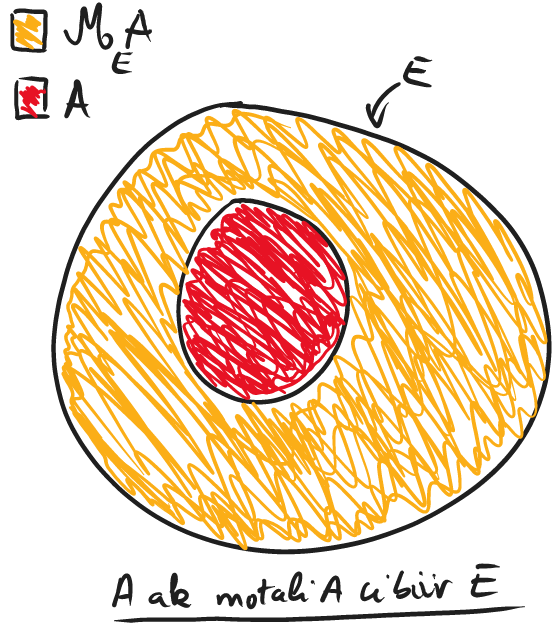
\includegraphics[scale = 0.5]{image/motali_emb.png}
  % \caption{}
  \label{fig:motali_emb}
\end{figure}
\begin{tcolorbox}[enhanced jigsaw,breakable,pad at break*=1mm, colback=orange!5!white,colframe=white!75!black,title= Seetlu,
    watermark color=white]
  Amal ëmb $A$ ab wàllu ëmb $E$. Bu féké ëmb bi di motali $A$ ci biir $E$ lu lér la, manaam munu ñu ko jaxasé ak leenen, kon mën nañu bindë $\Bar{A}$ ngir wax ëmb bi motali ci biir $E$.

  \begin{itemize}
    \item[$\bullet$] $\mathcal{M}_{E}A \cap A = \emptyset$, $\mathcal{M}_{E}(\mathcal{M}_{E}A) = A$
    \item[$\bullet$] $\mathcal{M}_{E}E = \emptyset$, $\mathcal{M}_{E}\emptyset = E$
  \end{itemize}
\end{tcolorbox}
\begin{tcolorbox}[enhanced jigsaw,breakable,pad at break*=1mm, colback=blue!5!white,colframe=white!75!black,title= Tèg\footnote{Proposition},
    watermark color=white]
  Amal ëmb $A$, $B$ ay wàllu ëmb $E$, kon
  \begin{align*}
    \mathcal{M}_{E}(A \cup B) & = (\mathcal{M}_{E}A) \cap (\mathcal{M}_{E}B)       \\
    \mathcal{M}_{E}(A \cap B) & = (\mathcal{M}_{E}A) \cup (\mathcal{M}_{E}B)       \\
    A \subset B               & \iff (\mathcal{M}_{E}B) \subset (\mathcal{M}_{E}A) \\
  \end{align*}
\end{tcolorbox}
\begin{figure}[ht]
  \centering
  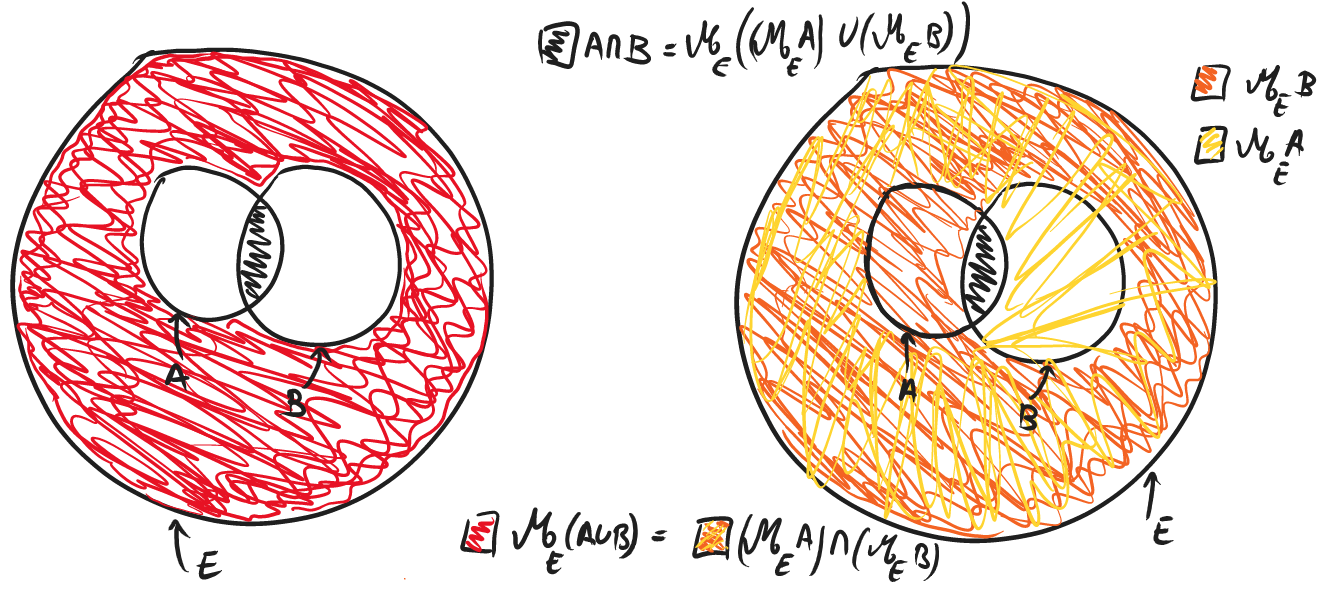
\includegraphics[scale = 0.5]{image/motali_emb_teg.png}
  % \caption{}
  \label{fig:motali_emb_teg}
\end{figure}

\subsection{Wañi ëmb ci ëmb}
\begin{tcolorbox}[enhanced jigsaw,breakable,pad at break*=1mm, colback=red!5!white,colframe=white!75!black,title= Téeki,watermark color=white]
  Amal ëmb $A$ ak $B$ ay wàllu been ëmb $E$, \textbf{ëmb bi di motali $B$ ci biir $A$}, ñu di ko bindë $$A - B = \big \{x \in E, \text{ té } x \in A \text{ ak } x \not \in B\}$$
  mo di saamu ëmbeef yëp yu nék ci $A$ té nekku ñu ci $B$. Yèna say ñu bindé ko $A \backslash B$
\end{tcolorbox}

\begin{tcolorbox}[enhanced jigsaw,breakable,pad at break*=1mm, colback=orange!5!white,colframe=white!75!black,title= Seetlu,
    watermark color=white]
  Amal ëmb $A$ ak $B$ ay wàllu been ëmb $E$, boba
  \begin{itemize}
    \item[$\bullet$] $A\backslash B = \mathcal{M}_A (A\cap B) = A \cap \mathcal{M}_E (B)$
  \end{itemize}
\end{tcolorbox}
\textbf{Rëd fi been natal bu di mandargal kaadu yi muj.}

\begin{tcolorbox}[enhanced jigsaw,breakable,pad at break*=1mm, colback=red!5!white,colframe=white!75!black,title= Téeki,watermark color=white]
  Amal ëmb $A$ ak $B$ ay wàllu been ëmb $E$, \textbf{wuté simetiri ci diganté $A$ ak $B$}\footnote{différence symétrique
  }, ñu di ko bindë $$A \Delta  B = (A-B) \cup (B-A)$$
  mo di saamu ëmbeef yëp yu nék ci $A$ té nekku ñu ci $B$.
\end{tcolorbox}

\begin{tcolorbox}[enhanced jigsaw,breakable,pad at break*=1mm, colback=orange!5!white,colframe=white!75!black,title= Seetlu,
    watermark color=white]
  Amal ëmb $A$ ak $B$ ay wàllu been ëmb $E$, boba
  \begin{itemize}
    \item[$\bullet$] $A \Delta  B = (A \cup B) \backslash (A \cap B)$
  \end{itemize}
\end{tcolorbox}
\textbf{Rëd fi been natal bu di mandargal kaadu yi muj.}


\subsection{Njabootu ay ëmbeef}
\begin{tcolorbox}[enhanced jigsaw,breakable,pad at break*=1mm, colback=red!5!white,colframe=white!75!black,title= Téeki,watermark color=white]
  Njabbotu ay ëmbeefu been ëmb $E$, mo di beep mbir gi joxé been ëmbeef $x_i \in E$ ak beep $i$ ci biir been ëmb $I$, ñu di ko bindé $(x_i)_{i\in I}$.

  $E^I$ la ñuy bindé njabootu ëmb yëp yu joxé been ëmbeef $x_i \in E$ ak beep $i$ ci biir been ëmb $I$. $I$ moy ëmb bi di ràññee ëmbeefu $E$ yi ci njabboot $(x_i)_{i\in I}$.
\end{tcolorbox}
\begin{tcolorbox}[enhanced jigsaw,breakable,pad at break*=1mm, colback=orange!5!white,colframe=white!75!black,title= Seetlu,
    watermark color=white]
  Bu féké limu ëmbeef yu bok ci $I$ day jex $I$\footnote{$I$ est un ensemble fini.}, boba beep njabootu ay ëmbeefu $E$ itam di na jex.

  Bu féké $I=\N$, kon beep njabbootu $E^I$ \textbf{topalanté} la ñu koy wowé.
\end{tcolorbox}

\end{document}
